% !TEX root = ../main.tex

\section{Method}
\label{sec:orga8a42f5}
\label{section:method}

In this section, we introduce our approach for multilabel problems, with a Confusion Matrix Metric as a loss. In evaluation of multilabel or multiclass problems, confusion matrix metrics are a common choice, because they implicitly deal with label count. In our framework, we leverage a smoothed version of the confusion matrix that can be used to directly optimize as a loss function (the original confusion matrix metrics rely on step functions and are therefore intractable). Before we discuss smoothing the confusion matrix metrics, we first briefly recap our learning setting and define the confusion matrix metrics in this setting more formally.

\begin{figure}[tbp]
\centering
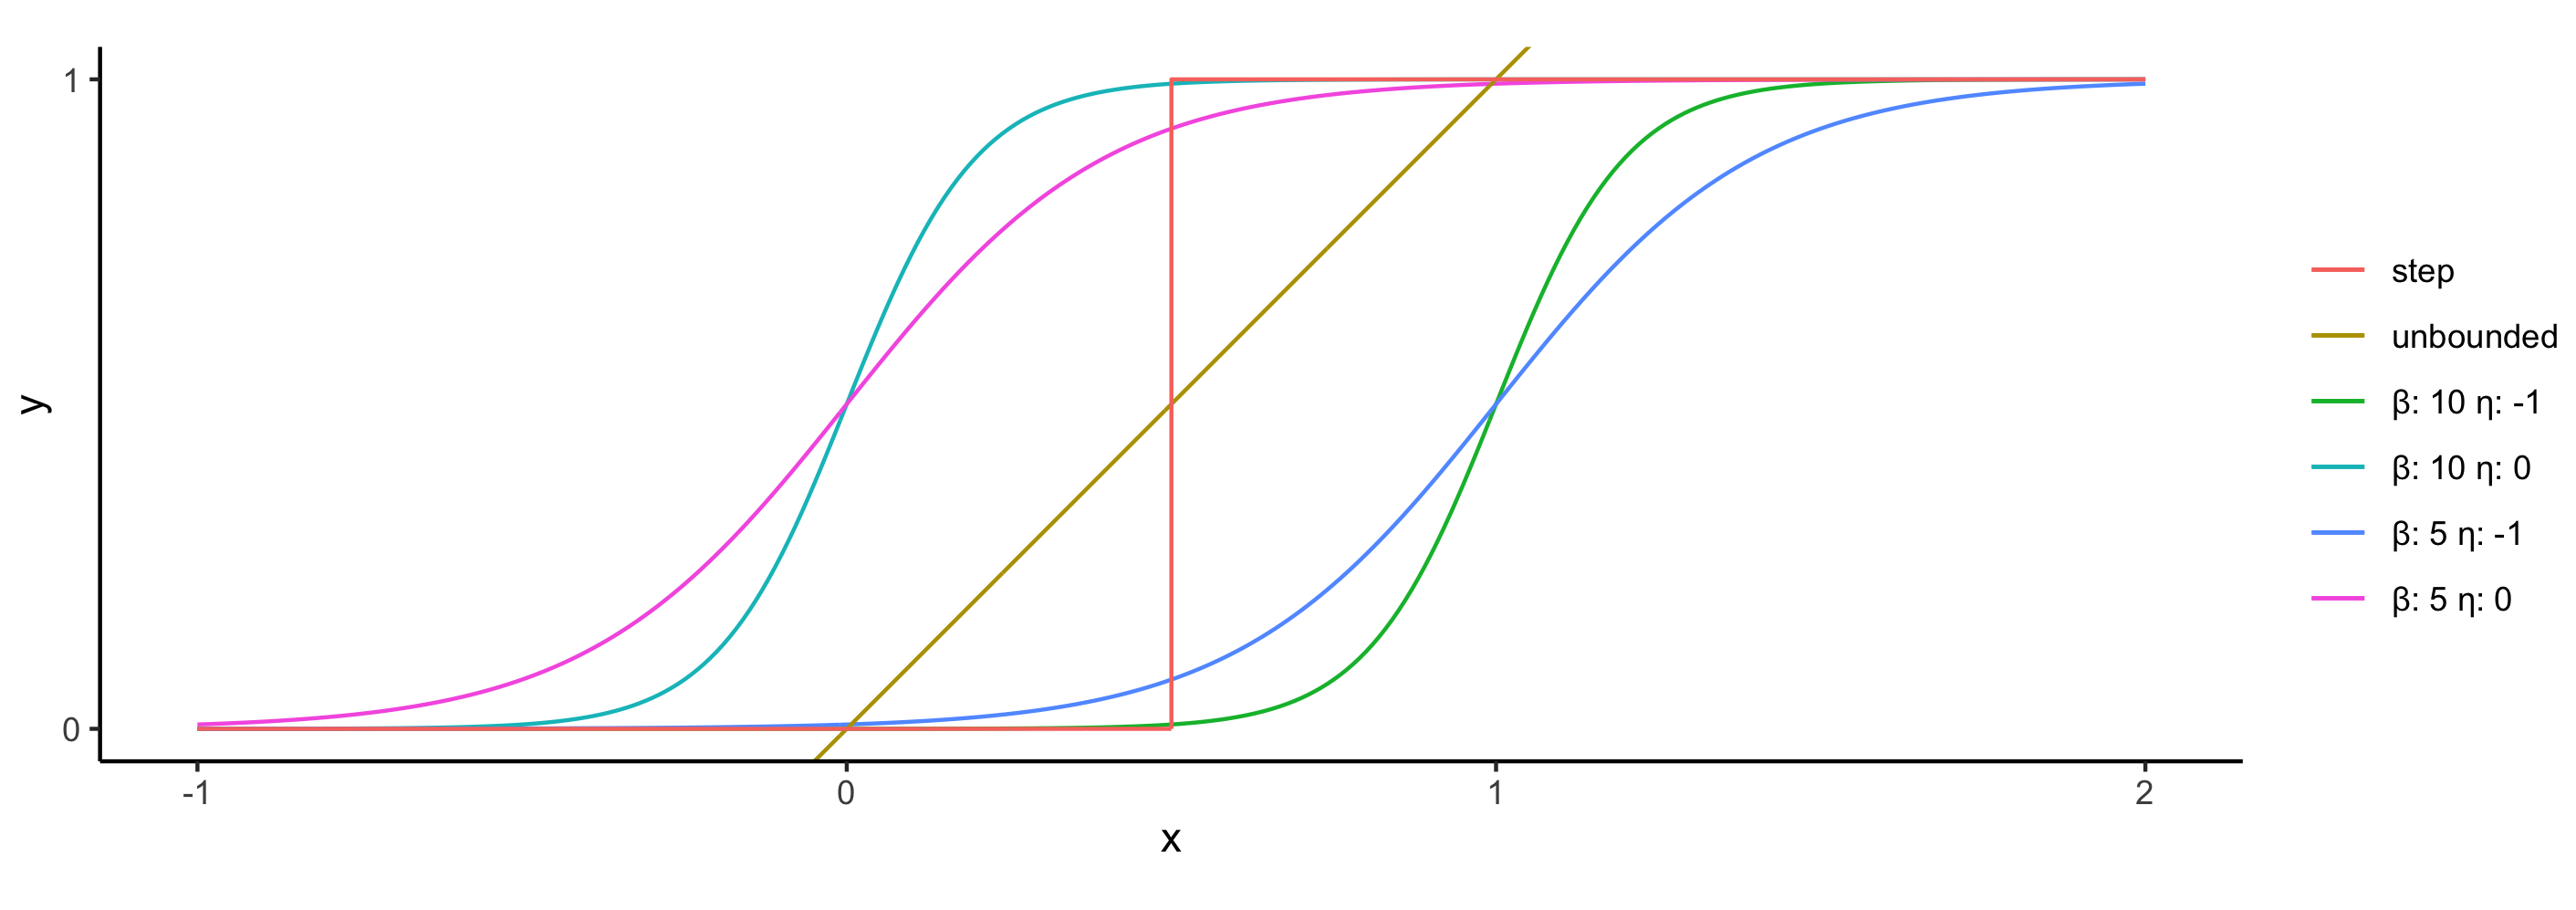
\includegraphics[width=\linewidth]{./images/sigmoid.png}
\caption{\label{fig:sigmoid}
Different thresholding regimes: the non-decomposable step function, the unbounded linear function and the sigmoid function at different parametrizations}\todo{Redraw for single column.}
\end{figure}
\label{fig:sigmoid}

% For the same class of learning algorithms defined in the previous section \(\mathcal{F}(\cdot ; \Theta): \mathcal{X} \rightarrow \mathcal{Y}\), we consider a particular case, where \(\mathbf{x} = \{x_1, \ldots, x_n\}\) and each observation is assigned $k$ labels (one or more) \(\mathbf{l} = \{l_1, \ldots, l_C\}\) out of a set of classes $C$. \(y_{i}^{j}\) are binary variables, indicating presence of a label for each observation \(i\) and class \(j\).

% For each observation \(i\), label class probabilities can be defined based on predictions as

% \todo{check this formula}

% \begin{equation}
% \mathbf{p}_{i}=\left\{\begin{array}{ll}\hat{\mathbf{y}} & \text { if } y=1 \\ 1-\hat{\mathbf{y}} & \text { otherwise }\end{array}\right.
% \end{equation}

We use the binary classification setting (two classes) as it simplifies the notation and prevents further use of subscripts or matrix operations, without loss of generalization to the multiclass case.
In a typical binary classification problem with the label vector $\mathbf{y} = \{y_1 , \ldots, y_n\}$, predictions are probabilistic and it is necessary to define a threshold \(t\), at which a prediction is dichotomized. With \(\mathds{1}\) as an indicator function, \(Y^+ = \sum \mathds{1}_{\hat{\mathbf{y}} \geq t}\), \(Y^- = \sum \mathds{1}_{\hat{\mathbf{y}} < t}\) are thus the count of positive and negative predictions at threshold \(t\). Let \(tp\), \(fp\), \(fn\), \(tn\) be number of true positives, false positives, false negatives and true negatives respectively:
%
\begin{equation}
\label{eq:conf}
\begin{array}{ll}\mathit{tp} = \sum \mathds{1}_{\hat{\mathbf{y}} \geq t} \odot \mathbf{y}  & \mathit{fp} = \sum \mathds{1}_{\hat{\mathbf{y}} \geq t} \odot (\mathds{1} - \mathbf{y}) \\[.5em] \mathit{fn} = \sum \mathds{1}_{\hat{\mathbf{y}} < t} \odot \mathbf{y} & \mathit{tn} = \sum \mathds{1}_{\hat{\mathbf{y}} < t} \odot (\mathds{1} - \mathbf{y}),
\end{array}
\end{equation}
%
%, \(\sum^+\) and \(\sum^-\) corresponding to  \(\sum_{i \in Y^{+}}\) and \(\sum_{i \in Y^{-}}\) respectively
with \(\odot\) the component-wise multiplication sign.


For simplicity, in the formulation above and the ones that follow scores are calculated for a single class, therefore the sum is implicitly over all examples \(\sum_i\). This is useful for the binary classification problem but also for the multilabel problem, when micro metrics are calculated (i.e. metric for each class which is then averaged over all classes, see end of this section, where we further refine the micro and macro concepts). In the multilabel setting $\mathbf{y}$ can be substituted by $\mathbf{y}^j$ for each class $j$. Note that vectors could be trivially substituted by matrices ($Y$) in the following expressions to obtain the macro formulation.


% In the multilabel setting $\mathbf{y}$ can be substituted by $\mathbf{y}^j$ for each class $j$. Note that vectors could be trivially substituted by matrices ($Y$) in the following expressions to obtain the macro formulation.
% \doubt{do you agree that the subscript for the sum is implicit? and do you agree that the matrix formulation is trivial?}\hvk{do we really need this paragraph?}
% \daan{I think we should drop this.}

% Note that Equation \ref{eq:conf} represents a macro measure. For example, the micro $tp$ measure (i.e. for each class) would be $\sum \mathds{1}_{\hat{\mathbf{y}} \geq b} \odot \mathbf{y}$ $\sum_{i \in \hat{\mathbf{y}}^{j+}} \mathds{1}_{\hat{y}^{j}_{i} \geq b} \odot y^{j}_{i}$ (see end of this section, where we further refine the micro and macro concepts).

Given the four confusion matrix quadrants, we can generate further metrics like precision and recall (see Table \ref{tab:confusion-matrix}). However none of these metrics are decomposable due to the hard thresholding which is in effect a step function (see Figure \ref{fig:sigmoid}).

In the following sections, we first define desirable properties for decomposable thresholding.
Next, we define unbounded confusion matrix entries and a notion of sigmoid-based transformation that renders confusion matrix entries decomposable. Finally, we focus on an unbounded F1 score wich we use in our experiments.

\subsection{Desirable properties of decomposable thresholding}
\label{subsection:properties}

We thus define desirable properties for a decomposable sign function $f(u)$ as a surrogate of the above indicator function \(\mathds{1}_{\hat{\mathbf{y}} < t}\).

\begin{property}
  Boundedness: $|f(u)| < M$, where $M$ is an upper and lower bound.
\end{property}
The groundtruth $\mathbf{y}$ is bounded between $[0,1]$ and thus it must be compared to a bounded prediction $\mathbf{\hat{y}}$, preferably bounded by $[0,1]$, to avoid further scaling.

\begin{property}
  Saturation: $\int_{s}^{\infty} f^{-1}(u) = \int_{-\infty}^{-s} f(u) = \epsilon$, with $\epsilon$ a number close to zero and $s$ a saturation bound.
\end{property}
For the surrogate to be a proper sign function substitute, it is important to often return values close to 1 or 0. Saturation is defined in the context of neural network activation functions and refers to the propensity of iterative backpropagation to progressively lead to values very close to 0 or 1 after a long enough training period. While activation functions should tend to be non-saturated, in order for the derivative at point $u$ to be non-null and information to flow back to the network~\cite{saturation}, our sign function substitute must output values close to 0 or 1, in order to be comparable to a step function.

\begin{property}
  Dynamic Gradient: $f'(u) \gg 0 \quad \forall \; u \in [-s, s]$, where $s$ is the saturation bound.
\end{property}

Inside the saturation bounds $[-s, s]$, the derivative should be significantly higher than zero in order to facilitate stochastic gradient descent and backpropagation.

Note that the upper and lower limits of $f(u)$ are interchangeably $[-1,1]$ or $[0,1]$ along this paper and in the literature. The conditions above still apply by linear transformation.

In the following we show how our formalization of an unbounded F1 surrogate would not fulfill these properties and how our proposition of smooth bounded alternative does.


\subsection{Unbounded confusion matrix entries}
\label{subsec:unbounded}

A first trivial remedy to allow for derivation of the sign function, is to define \emph{unbounded} confusion matrix entries by replacing the dichotomized predictions with prediction probabilities. This way,
 (i.e. \(\overline{tp}\), \(\overline{fp}\), \(\overline{fn}\) and  \(\overline{tn}\) are not natural numbers anymore):
%
\begin{equation}
\label{eq:unbounded}
\begin{array}{ll} \overline{\mathit{tp}} = \sum \hat{\mathbf{y}} \odot \mathbf{y}  & \overline{\mathit{fp}} = \sum \hat{\mathbf{y}} \odot (\mathds{1} - \mathbf{y}) \\[.5em] \overline{\mathit{fn}} = \sum (\mathds{1} - \hat{\mathbf{y}}) \odot \mathbf{y} & \overline{\mathit{tn}} = \sum (\mathds{1} - \hat{\mathbf{y}}) \odot (\mathds{1} - \mathbf{y}),
\end{array}
\end{equation}
%
% $$
% \overline{tp}=\sum \hat{\mathbf{y}} \odot \mathbf{y} \quad \overline{fp} = \sum \hat{\mathbf{y}} \odot (\mathbf{1}- \mathbf{y}) \quad \overline{fn} = \sum (\mathbf{1} - \hat{\mathbf{y}}) \odot \mathbf{y}
% $$

\(tp\), \(fp\), \(fn\) and \(tn\) are now replaced by rough surrogates. The disadvantages are that the desirable properties mentioned above are not fulfilled, namely (i) \(\hat{\mathbf{y}}\) is unbounded and thus certain examples can have over-proportional effects on the loss, (ii) It is non-saturated. While non-saturation is desirable for activation functions~\cite{saturation}, it would be here desirable to tend towards saturation (i.e. tend to values close to 0 or 1, so as to give the most accurate predictions at any thresholding values at inference time). (iii) The gradient of that linear function is 1 and therefore backpropagation will not learn depending on different inputs at this stage of the loss function.

However, this method has the advantage of resulting in a linear loss function that avoids the concept of thresholding altogether and is trivial to decompose for stochastic gradient descent.

\subsection{Smooth confusion matrix entries}

We propose a sigmoid-based transformation of the confusion matrix that renders its entries decomposable and fulfills the three properties above:
%
\begin{equation}
\label{eq:smooth}
\begin{array}{ll} \widetilde{\mathit{tp}} = \sum \mathbf{S}(\hat{\mathbf{y}}) \odot \mathbf{y}  & \widetilde{\mathit{fp}} = \sum \mathbf{S}(\hat{\mathbf{y}}) \odot (\mathds{1} - \mathbf{y}) \\[.5em] \widetilde{\mathit{fn}} = \sum (\mathds{1} - \mathbf{S}(\hat{\mathbf{y}})) \odot \mathbf{y} & \widetilde{\mathit{tn}} = \sum (\mathds{1} - \mathbf{S}(\hat{\mathbf{y}})) \odot (\mathds{1} - \mathbf{y}),
\end{array}
\end{equation}
%
with $\mathbf{S}(\cdot)$ the vectorial form of the sigmoid function $S(\cdot)$:
%
\begin{equation}
S(u; \beta, \eta)=\frac{1}{1+\exp (-\beta (u + \eta))},
\end{equation}
%
with \(\beta\) and \(\eta\) tunable parameters for slope and offset respectively. Higher \(\beta\) results in steeper slope at the center of the sigmoid and thus more stringent thresholding. At its extreme, \(\lim_{\beta\to\infty} S(u; \beta, \eta)\) corresponds to the step function used in Equation \ref{eq:conf}. Note that negative values of $\beta$ geometrically reflect the sigmoid function across the horizontal line at $0.5$ and thus invert predictions.


These smooth confusion matrix entries allow to build any related metric (see Table \ref{tab:confusion-matrix}). Furthermore, the surrogate entries are decomposable, bounded, saturated and have a dynamic gradient.

\begin{table*}[]
\caption{Confusion matrix with our proposed smoothed confusion matrix entries, $\widetilde{\mathit{tp}}$, $\widetilde{\mathit{fp}}$, $\widetilde{\mathit{fn}}$ and $\widetilde{\mathit{tn}}$ and six derived loss functions that use these smoothed confusion matrix entries. $\mathcal{L}_{\widetilde{\mathit{F1}}}$ is used in our experiments.}
\label{tab:confusion-matrix}
\def\arraystretch{1.1}
\begin{tabular}{|c||c|c||c|} \cline{2-4}
\multicolumn{1}{l|}{} & \textbf{Condition} & \textbf{Condition} & \multirow{2}{*}{$\mathcal{L}_{\widetilde{\mathit{Accuracy}}}= \frac{\widetilde{\mathit{tp}} + \widetilde{\mathit{tn}}}{\widetilde{\mathit{tp}} + \widetilde{\mathit{fp}} + \widetilde{\mathit{tn}} + \widetilde{\mathit{fn}}}$} \\
\multicolumn{1}{l|}{} & \textbf{positive} &  \textbf{negative} & \\ \hline \hline
\textbf{~Predicted~} & True positive & False positive & \multirow{2}{*}{$\mathcal{L}_{\widetilde{\mathit{Precision}}}= \frac{\widetilde{\mathit{tp}}}{\widetilde{\mathit{tp}} + \widetilde{\mathit{fp}}}$} \\
\textbf{positive} & $\widetilde{\mathit{tp}}=\sum \mathbf{S}(\hat{\mathbf{y}}) \odot \mathbf{y}$ & $\widetilde{\mathit{fp}}= \sum \mathbf{S}(\hat{\mathbf{y}}) \odot (\mathds{1} - \mathbf{y})$ & \\ \hline
\textbf{Predicted} & False negative & True Negative & \multirow{2}{*}{$\mathcal{L}_{\widetilde{\mathit{NPV}}}= \frac{\widetilde{\mathit{tn}}}{\widetilde{\mathit{tn}} + \widetilde{\mathit{fn}}}$} \\
\textbf{negative} & $\widetilde{\mathit{fn}}= \sum (\mathds{1} - \mathbf{S}(\hat{\mathbf{y}})) \odot \mathbf{y}$ & $\widetilde{\mathit{tn}}= \sum (\mathds{1} - \mathbf{S}(\hat{\mathbf{y}})) \odot (\mathds{1} - \mathbf{y})$ & \\ \hline \hline
\multicolumn{1}{l|}{} & \multirow{2}{*}{\hspace{1.2em}$\mathcal{L}_{\widetilde{\mathit{Recall}}}= \frac{\widetilde{\mathit{tp}}}{\widetilde{\mathit{tp}} + \widetilde{\mathit{fn}}}$\hspace{1.2em}}& \multirow{2}{*}{$\mathcal{L}_{\widetilde{\mathit{Specificity}}}= \frac{\widetilde{\mathit{tn}}}{\widetilde{\mathit{fp}} + \widetilde{\mathit{tn}}}$} & \multirow{2}{*}{$\mathcal{L}_{\widetilde{\mathit{F1}}}= \frac{\widetilde{\mathit{tp}}}{2 \widetilde{\mathit{tp}}+ \widetilde{\mathit{fn}}+ \widetilde{\mathit{fp}}}$} \\
\multicolumn{1}{l|}{} & & & \\
\cline{2-4}
\end{tabular}%
\end{table*}

In this paper we focus on sigmoidF1 ($\mathcal{L}_{\widetilde{\mathit{F1}}}$) because it has the ability to implicitly penalize for both inacurate label propensity and label count.


\subsection{Smooth macro F1 scores}
\label{sec:orgc5d29d7}

While smoothness is defined above, there is yet a precision to make about micro-averaging versus macro-averaging in multilabel-classification problems. Micro-averaging is biased by class frequency, whereas macro-averaging regards all classes as equally important. \emph{unboundedF1} and \emph{sigmoidF1} below are thought of as macro scores (aggregated over all classes). These scores require a high enough number of representatives in the four confusion matrix quadrants to learn from batch to batch. Ideally, each training epoch would have only one batch, so as to have the most representatives.

Following Equation \ref{eq:unbounded}, it is possible to define an \emph{unbounded F1} score. A formulation similar to \emph{unboundedF1} was proposed in an unpublished blog post, which was referred to as \emph{softF1}~\cite{softF1}. We define our \emph{unbounded F1} score as follows:
%
\begin{equation}
\mathcal{L}_{\overline{\mathit{F1}}}= \frac{\overline{tp}}{2 \overline{tp}+ \overline{fn}+ \overline{fp}}
\end{equation}
%
While this alternative abstracts the thresholding away, which is convenient for fine-tuning purposes, it does not fulfil the desirable properties of a dichotomization threshold surrogate. For more on that see Section~\ref{subsec:unbounded}.

\emph{unboundedF1} will be used to benchmark against our proposed \emph{sigmoidF1} loss. Given the definitions of smooth confusion matrix metrics above, we can now write $\mathcal{L}_{\widetilde{\mathit{F1}}}$.
%
\begin{equation}\label{eq:sigmoidF1}
\mathcal{L}_{\widetilde{\mathit{F1}}}= \frac{\widetilde{\mathit{tp}}}{2 \widetilde{\mathit{tp}}+ \widetilde{\mathit{fn}}+ \widetilde{\mathit{fp}}}
\end{equation}
%
A similar method was proposed outside of the context of neural networks: the \emph{Maximum F1-score criterion} for automatic mispronunciation detection as an objective function to a Gaussian Mixture Model-hidden Markov model (GMM-HMM)\cite{sigmoid}.

\emph{sigmoidF1} is particularly suited for the multilabel setting because it is a proper hard thresholding surrogate as defined in the previous sections and because it contains a significant amount of information about label prediction accuracy: $\widetilde{\mathit{tp}}$, $\widetilde{\mathit{fn}}$ and $\widetilde{\mathit{fp}}$ are indicative of the number of predicted labels in each category of the confusion matrix but also contain a notion of certainty, given that they are rational numbers. The built in sigmoid function ensures that certainty increases along training epochs, as outlined by proposition 2. Finally, as the harmonic mean of precision and recall (A property of F1 in general), it weighs in both relevance metrics.

\vspace{\baselineskip}

We end this section by writing down the focal loss~\cite{focalLoss}, as it deals specifically with class imbalance and is used as a benchmark due to its popularity in the multiclass domain.
%
\begin{equation}
  \mathcal{L}_{FL} = -\alpha^{\mathrm{j}}\left(1-\hat{y}^{\mathrm{j}}\right)^{\gamma} \log \left(\hat{y}^{\mathrm{j}}\right),
\end{equation}
%
with $\alpha^j$ and $\gamma$ hyperparameters. In the next section, we further specify the setup for focal loss and cross entropy as benchmarks for \emph{unboundedF1} and \emph{sigmoidF1}.

% Given the presence of the step indicator function \(\sum \mathds{1}_{\mathbf{p_i} \geq b}\), \(F_\beta\) is not differentiable for gradient based methods. One way of surpassing that problem is to use a surrogate.

% \subsection{soft F1 score}
% \label{sec:org3ca83ef}

 % with smooth confusion matrix entries :



% /softF1/ is
% $$\mathcal{L}_{\text {Pred}}=\sum_{i, j}\left(\mathbf{y}_{i j}-\hat{\mathbf{y}}_{i j}\right)^{2}$$

% \subsection{sigmoidF1 score}
% \label{sec:orgc5d29d7}


% \begin{figure}[htbp]
% \centering
% 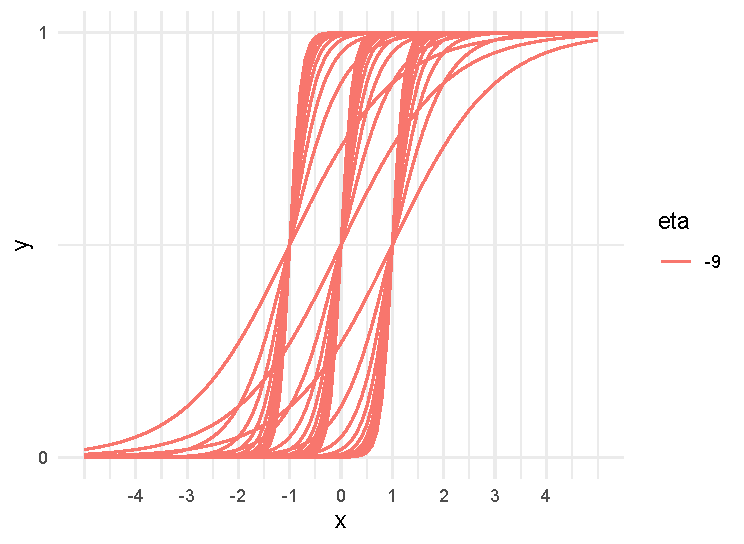
\includegraphics[width=.9\linewidth]{./images/sigmoid.pdf}
% \caption{\label{fig:sigmoid}
% Sigmoid function with different values for $\beta$ (steepness) \& $\eta$ (offset)}
% \end{figure}

%  with \(S(u)\), the confusion matrix entries then become

% \begin{equation}\label{eq:sigmoidF1}
% \widetilde{\mathit{tp}}=\sum S(\hat{\mathbf{y}}) \odot \mathbf{y} \quad\widetilde{\mathit{fp}}= \sum S(\hat{\mathbf{y}}) \odot (\mathbf{1} - \mathbf{y}) \quad \widetilde{\mathit{fn}}= \sum (\mathbf{1} - S(\hat{\mathbf{y}})) \odot \mathbf{y}
% \end{equation}

% And thus

% \begin{equation}
% \mathcal{L}_{\text {sigmoidF1}}= \frac{\widetilde{\mathit{tp}}}{2 \widetilde{\mathit{tp}}+ \widetilde{\mathit{fn}}+ \widetilde{\mathit{fp}}}
% \end{equation}

% \doubt{mention smooth hinge loss} \cite{smoothHinge}

% $\doublewidetilde{tp}$
% https://tex.stackexchange.com/questions/321231/double-widetilde
% doesn't work


% \todo{explain batch size mathematically for F1 surrogate losses}


%%% Local Variables:
%%% mode: latex
%%% TeX-master: "../main"
%%% End:
